
\documentclass[11pt,a4paper,oneside]{report}

\usepackage{float}
\usepackage{tikz}
\usetikzlibrary{plotmarks}
\usepackage{amsmath,graphicx}
\usepackage{epstopdf}
\usepackage[font=normal,labelfont=bf]{caption}
\usepackage{subcaption}
\usepackage{color}
\usepackage[T1]{fontenc}
\usepackage{lmodern}
\usepackage{scalefnt}


% margin size
\usepackage[margin=1in]{geometry}

% tikz settings
\tikzstyle{state}=[circle,thick,draw=black, align=center, minimum size=2.1cm,
inner sep=0]
\tikzstyle{vertex}=[circle,thick,draw=black]
\tikzstyle{terminal}=[rectangle,thick,draw=black]
\tikzstyle{edge} = [draw,thick]
\tikzstyle{lo} = [edge,dotted]
\tikzstyle{hi} = [edge]
\tikzstyle{trans} = [edge,->]


\begin{document}
\belowdisplayskip=12pt plus 3pt minus 9pt
\belowdisplayshortskip=7pt plus 3pt minus 4pt

% scale parameter for the circles and the gradient
\tikzset{every picture/.append style={scale=0.6}}
% scale parameter for the upper and lower small brain images
\newcommand*{\scaleBrainImg}{0.3}

%col{x}{y}{z} respresents the color for ball z from matrix x at stage y (matrix x, stage y, ball z)

\definecolor{col000_2}{rgb}{1,0.000,0}
\definecolor{col001_2}{rgb}{1,0.136,0}
\definecolor{col002_2}{rgb}{1,0.032,0}
\definecolor{col003_2}{rgb}{1,0.000,0}
\definecolor{col004_2}{rgb}{1,0.002,0}
\definecolor{col005_2}{rgb}{1,0.026,0}
\definecolor{col006_2}{rgb}{1,1.000,0}
\definecolor{col010_2}{rgb}{1,0.000,0}
\definecolor{col011_2}{rgb}{1,0.000,0}
\definecolor{col012_2}{rgb}{1,0.000,0}
\definecolor{col013_2}{rgb}{1,0.000,0}
\definecolor{col014_2}{rgb}{1,0.000,0}
\definecolor{col015_2}{rgb}{1,0.000,0}
\definecolor{col016_2}{rgb}{1,0.002,0}
\definecolor{col020_2}{rgb}{1,0.000,0}
\definecolor{col021_2}{rgb}{1,0.000,0}
\definecolor{col022_2}{rgb}{1,0.000,0}
\definecolor{col023_2}{rgb}{1,0.000,0}
\definecolor{col024_2}{rgb}{1,0.000,0}
\definecolor{col025_2}{rgb}{1,0.000,0}
\definecolor{col026_2}{rgb}{1,0.000,0}
\definecolor{col030_2}{rgb}{1,0.000,0}
\definecolor{col031_2}{rgb}{1,0.000,0}
\definecolor{col032_2}{rgb}{1,0.000,0}
\definecolor{col033_2}{rgb}{1,0.000,0}
\definecolor{col034_2}{rgb}{1,0.000,0}
\definecolor{col035_2}{rgb}{1,0.000,0}
\definecolor{col036_2}{rgb}{1,0.000,0}
\definecolor{col040_2}{rgb}{1,0.000,0}
\definecolor{col041_2}{rgb}{1,0.000,0}
\definecolor{col042_2}{rgb}{1,0.000,0}
\definecolor{col043_2}{rgb}{1,0.000,0}
\definecolor{col044_2}{rgb}{1,0.000,0}
\definecolor{col045_2}{rgb}{1,0.000,0}
\definecolor{col046_2}{rgb}{1,0.000,0}
\definecolor{col100_2}{rgb}{1,0.325,0}
\definecolor{col101_2}{rgb}{1,0.586,0}
\definecolor{col102_2}{rgb}{1,0.189,0}
\definecolor{col103_2}{rgb}{1,0.355,0}
\definecolor{col104_2}{rgb}{1,0.443,0}
\definecolor{col105_2}{rgb}{1,0.510,0}
\definecolor{col106_2}{rgb}{1,0.702,0}
\definecolor{col110_2}{rgb}{1,0.080,0}
\definecolor{col111_2}{rgb}{1,0.216,0}
\definecolor{col112_2}{rgb}{1,0.038,0}
\definecolor{col113_2}{rgb}{1,0.100,0}
\definecolor{col114_2}{rgb}{1,0.123,0}
\definecolor{col115_2}{rgb}{1,0.151,0}
\definecolor{col116_2}{rgb}{1,0.367,0}
\definecolor{col120_2}{rgb}{1,0.023,0}
\definecolor{col121_2}{rgb}{1,0.080,0}
\definecolor{col122_2}{rgb}{1,0.007,0}
\definecolor{col123_2}{rgb}{1,0.024,0}
\definecolor{col124_2}{rgb}{1,0.039,0}
\definecolor{col125_2}{rgb}{1,0.038,0}
\definecolor{col126_2}{rgb}{1,0.155,0}
\definecolor{col130_2}{rgb}{1,0.005,0}
\definecolor{col131_2}{rgb}{1,0.022,0}
\definecolor{col132_2}{rgb}{1,0.005,0}
\definecolor{col133_2}{rgb}{1,0.004,0}
\definecolor{col134_2}{rgb}{1,0.009,0}
\definecolor{col135_2}{rgb}{1,0.014,0}
\definecolor{col136_2}{rgb}{1,0.047,0}
\definecolor{col140_2}{rgb}{1,0.001,0}
\definecolor{col141_2}{rgb}{1,0.000,0}
\definecolor{col142_2}{rgb}{1,0.000,0}
\definecolor{col143_2}{rgb}{1,0.000,0}
\definecolor{col144_2}{rgb}{1,0.001,0}
\definecolor{col145_2}{rgb}{1,0.001,0}
\definecolor{col146_2}{rgb}{1,0.001,0}
\definecolor{col200_2}{rgb}{1,0.471,0}
\definecolor{col201_2}{rgb}{1,0.388,0}
\definecolor{col202_2}{rgb}{1,0.519,0}
\definecolor{col203_2}{rgb}{1,0.556,0}
\definecolor{col204_2}{rgb}{1,0.610,0}
\definecolor{col205_2}{rgb}{1,0.699,0}
\definecolor{col206_2}{rgb}{1,0.642,0}
\definecolor{col210_2}{rgb}{1,0.188,0}
\definecolor{col211_2}{rgb}{1,0.170,0}
\definecolor{col212_2}{rgb}{1,0.250,0}
\definecolor{col213_2}{rgb}{1,0.254,0}
\definecolor{col214_2}{rgb}{1,0.329,0}
\definecolor{col215_2}{rgb}{1,0.389,0}
\definecolor{col216_2}{rgb}{1,0.374,0}
\definecolor{col220_2}{rgb}{1,0.070,0}
\definecolor{col221_2}{rgb}{1,0.065,0}
\definecolor{col222_2}{rgb}{1,0.119,0}
\definecolor{col223_2}{rgb}{1,0.113,0}
\definecolor{col224_2}{rgb}{1,0.168,0}
\definecolor{col225_2}{rgb}{1,0.185,0}
\definecolor{col226_2}{rgb}{1,0.182,0}
\definecolor{col230_2}{rgb}{1,0.030,0}
\definecolor{col231_2}{rgb}{1,0.032,0}
\definecolor{col232_2}{rgb}{1,0.050,0}
\definecolor{col233_2}{rgb}{1,0.052,0}
\definecolor{col234_2}{rgb}{1,0.084,0}
\definecolor{col235_2}{rgb}{1,0.088,0}
\definecolor{col236_2}{rgb}{1,0.073,0}
\definecolor{col240_2}{rgb}{1,0.001,0}
\definecolor{col241_2}{rgb}{1,0.007,0}
\definecolor{col242_2}{rgb}{1,0.007,0}
\definecolor{col243_2}{rgb}{1,0.003,0}
\definecolor{col244_2}{rgb}{1,0.011,0}
\definecolor{col245_2}{rgb}{1,0.011,0}
\definecolor{col246_2}{rgb}{1,0.005,0}
\definecolor{col300_2}{rgb}{1,1.000,0}
\definecolor{col301_2}{rgb}{1,0.998,0}
\definecolor{col302_2}{rgb}{1,1.000,0}
\definecolor{col303_2}{rgb}{1,0.960,0}
\definecolor{col304_2}{rgb}{1,0.809,0}
\definecolor{col305_2}{rgb}{1,0.944,0}
\definecolor{col306_2}{rgb}{1,0.986,0}
\definecolor{col310_2}{rgb}{1,1.000,0}
\definecolor{col311_2}{rgb}{1,0.994,0}
\definecolor{col312_2}{rgb}{1,1.000,0}
\definecolor{col313_2}{rgb}{1,0.890,0}
\definecolor{col314_2}{rgb}{1,0.537,0}
\definecolor{col315_2}{rgb}{1,0.843,0}
\definecolor{col316_2}{rgb}{1,0.960,0}
\definecolor{col320_2}{rgb}{1,0.997,0}
\definecolor{col321_2}{rgb}{1,0.988,0}
\definecolor{col322_2}{rgb}{1,1.000,0}
\definecolor{col323_2}{rgb}{1,0.756,0}
\definecolor{col324_2}{rgb}{1,0.302,0}
\definecolor{col325_2}{rgb}{1,0.660,0}
\definecolor{col326_2}{rgb}{1,0.895,0}
\definecolor{col330_2}{rgb}{1,0.987,0}
\definecolor{col331_2}{rgb}{1,0.971,0}
\definecolor{col332_2}{rgb}{1,1.000,0}
\definecolor{col333_2}{rgb}{1,0.508,0}
\definecolor{col334_2}{rgb}{1,0.160,0}
\definecolor{col335_2}{rgb}{1,0.448,0}
\definecolor{col336_2}{rgb}{1,0.779,0}
\definecolor{col340_2}{rgb}{1,0.827,0}
\definecolor{col341_2}{rgb}{1,0.655,0}
\definecolor{col342_2}{rgb}{1,0.953,0}
\definecolor{col343_2}{rgb}{1,0.043,0}
\definecolor{col344_2}{rgb}{1,0.014,0}
\definecolor{col345_2}{rgb}{1,0.099,0}
\definecolor{col346_2}{rgb}{1,0.177,0}

 
\begin{figure}[H]
  \centering
  %\begin{subfigure}[b]{0.15\textwidth}
    \begin{tikzpicture}[scale=1.0,auto,swap]

    % the two brain figures on top
    \node (upper_brain) at (0,1.5) { \includegraphics*[scale=\scaleBrainImg,trim=0 0 240 0]{images/GMM_2/stage_6.eps}};
    \node (lower_brain) at (0,-1.5) { \includegraphics*[scale=\scaleBrainImg,trim=240 0 0 0]{images/GMM_2/stage_6.eps}};

    % the 6 circles
    \draw[fill=col000_2] (-1.6,-3.4) circle [radius=0.33cm] node {\scriptsize A};
    \draw[fill=col001_2] (-0.7,-3.4) circle [radius=0.33cm] node {\scriptsize P};
    \draw[fill=col002_2] (0.2,-3.4) circle [radius=0.33cm] node {\scriptsize T};
    \draw[fill=col003_2] (-1.6,-4.2) circle [radius=0.33cm] node {\scriptsize C1};
    \draw[fill=col004_2] (-0.7,-4.2) circle [radius=0.33cm] node {\scriptsize C2};
    \draw[fill=col005_2] (0.2,-4.2) circle [radius=0.33cm] node {\scriptsize C3};

    % the big circle on the right
    \draw[fill=col006_2] (1.3,-3.8) circle [radius=0.6cm] node {\scriptsize FDG};

    \end{tikzpicture}
  %\end{subfigure}
  % next subfigure
  \hspace{-1.5em}
  ~
  %\begin{subfigure}[b]{0.15\textwidth}
    \begin{tikzpicture}[scale=1.0,auto,swap]

    % the two brain figures on top
    \node (upper_brain) at (0,1.5) { \includegraphics*[scale=\scaleBrainImg,trim=0 0 240 0]{images/GMM_2/stage_12.eps}};
    \node (lower_brain) at (0,-1.5) { \includegraphics*[scale=\scaleBrainImg,trim=240 0 0 0]{images/GMM_2/stage_12.eps}};

    % the 6 circles
    \draw[fill=col010_2] (-1.6,-3.4) circle [radius=0.33cm] node {\scriptsize A};
    \draw[fill=col011_2] (-0.7,-3.4) circle [radius=0.33cm] node {\scriptsize P};
    \draw[fill=col012_2] (0.2,-3.4) circle [radius=0.33cm] node {\scriptsize T};
    \draw[fill=col013_2] (-1.6,-4.2) circle [radius=0.33cm] node {\scriptsize C1};
    \draw[fill=col014_2] (-0.7,-4.2) circle [radius=0.33cm] node {\scriptsize C2};
    \draw[fill=col015_2] (0.2,-4.2) circle [radius=0.33cm] node {\scriptsize C3};

    % the big circle on the right
    \draw[fill=col016_2] (1.3,-3.8) circle [radius=0.6cm] node {\scriptsize FDG};

    \end{tikzpicture}
  %\end{subfigure}
  % next subfigure
  \hspace{-1.5em}
  ~
  %\begin{subfigure}[b]{0.15\textwidth}
    \begin{tikzpicture}[scale=1.0,auto,swap]

    % the two brain figures on top
    \node (upper_brain) at (0,1.5) { \includegraphics*[scale=\scaleBrainImg,trim=0 0 240 0]{images/GMM_2/stage_18.eps}};
    \node (lower_brain) at (0,-1.5) { \includegraphics*[scale=\scaleBrainImg,trim=240 0 0 0]{images/GMM_2/stage_18.eps}};

    % the 6 circles
    \draw[fill=col020_2] (-1.6,-3.4) circle [radius=0.33cm] node {\scriptsize A};
    \draw[fill=col021_2] (-0.7,-3.4) circle [radius=0.33cm] node {\scriptsize P};
    \draw[fill=col022_2] (0.2,-3.4) circle [radius=0.33cm] node {\scriptsize T};
    \draw[fill=col023_2] (-1.6,-4.2) circle [radius=0.33cm] node {\scriptsize C1};
    \draw[fill=col024_2] (-0.7,-4.2) circle [radius=0.33cm] node {\scriptsize C2};
    \draw[fill=col025_2] (0.2,-4.2) circle [radius=0.33cm] node {\scriptsize C3};

    % the big circle on the right
    \draw[fill=col026_2] (1.3,-3.8) circle [radius=0.6cm] node {\scriptsize FDG};

    \end{tikzpicture}
  %\end{subfigure}
  % next subfigure
  \hspace{-1.5em}
  ~
  %\begin{subfigure}[b]{0.15\textwidth}
    \begin{tikzpicture}[scale=1.0,auto,swap]

    % the two brain figures on top
    \node (upper_brain) at (0,1.5) { \includegraphics*[scale=\scaleBrainImg,trim=0 0 240 0]{images/GMM_2/stage_24.eps}};
    \node (lower_brain) at (0,-1.5) { \includegraphics*[scale=\scaleBrainImg,trim=240 0 0 0]{images/GMM_2/stage_24.eps}};

    % the 6 circles
    \draw[fill=col030_2] (-1.6,-3.4) circle [radius=0.33cm] node {\scriptsize A};
    \draw[fill=col031_2] (-0.7,-3.4) circle [radius=0.33cm] node {\scriptsize P};
    \draw[fill=col032_2] (0.2,-3.4) circle [radius=0.33cm] node {\scriptsize T};
    \draw[fill=col033_2] (-1.6,-4.2) circle [radius=0.33cm] node {\scriptsize C1};
    \draw[fill=col034_2] (-0.7,-4.2) circle [radius=0.33cm] node {\scriptsize C2};
    \draw[fill=col035_2] (0.2,-4.2) circle [radius=0.33cm] node {\scriptsize C3};

    % the big circle on the right
    \draw[fill=col036_2] (1.3,-3.8) circle [radius=0.6cm] node {\scriptsize FDG};

    \end{tikzpicture}
  %\end{subfigure}
  % next subfigure
  \hspace{-1.5em}
  ~
  %\begin{subfigure}[b]{0.15\textwidth}
    \begin{tikzpicture}[scale=1.0,auto,swap]

    % the two brain figures on top
    \node (upper_brain) at (0,1.5) { \includegraphics*[scale=\scaleBrainImg,trim=0 0 240 0]{images/GMM_2/stage_36.eps}};
    \node (lower_brain) at (0,-1.5) { \includegraphics*[scale=\scaleBrainImg,trim=240 0 0 0]{images/GMM_2/stage_36.eps}};

    % the 6 circles
    \draw[fill=col040_2] (-1.6,-3.4) circle [radius=0.33cm] node {\scriptsize A};
    \draw[fill=col041_2] (-0.7,-3.4) circle [radius=0.33cm] node {\scriptsize P};
    \draw[fill=col042_2] (0.2,-3.4) circle [radius=0.33cm] node {\scriptsize T};
    \draw[fill=col043_2] (-1.6,-4.2) circle [radius=0.33cm] node {\scriptsize C1};
    \draw[fill=col044_2] (-0.7,-4.2) circle [radius=0.33cm] node {\scriptsize C2};
    \draw[fill=col045_2] (0.2,-4.2) circle [radius=0.33cm] node {\scriptsize C3};

    % the big circle on the right
    \draw[fill=col046_2] (1.3,-3.8) circle [radius=0.6cm] node {\scriptsize FDG};

    \end{tikzpicture}
  %\end{subfigure}
  % next subfigure
  \hspace{-1.5em}
  ~
  \hspace{1em}
  % the red-to-yellow gradient on the right
  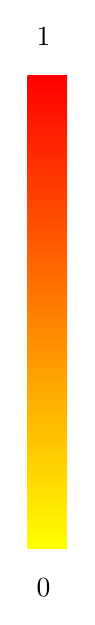
\begin{tikzpicture}[scale=1.0,auto,swap]
    \shade[top color=red,bottom color=yellow] (0,0) rectangle (0.5,6);
    \node[inner sep=0] (corr_text) at (0.2,6.5) {1};
    \node[inner sep=0] (corr_text) at (0.2,-0.5) {0};
  \end{tikzpicture}
  \caption{GMM}
\end{figure}


\begin{figure}[H]
  \centering
  %\begin{subfigure}[b]{0.15\textwidth}
    \begin{tikzpicture}[scale=1.0,auto,swap]

    % the two brain figures on top
    \node (upper_brain) at (0,1.5) { \includegraphics*[scale=\scaleBrainImg,trim=0 0 240 0]{images/cluster1_2/stage_6.eps}};
    \node (lower_brain) at (0,-1.5) { \includegraphics*[scale=\scaleBrainImg,trim=240 0 0 0]{images/cluster1_2/stage_6.eps}};

    % the 6 circles
    \draw[fill=col100_2] (-1.6,-3.4) circle [radius=0.33cm] node {\scriptsize A};
    \draw[fill=col101_2] (-0.7,-3.4) circle [radius=0.33cm] node {\scriptsize P};
    \draw[fill=col102_2] (0.2,-3.4) circle [radius=0.33cm] node {\scriptsize T};
    \draw[fill=col103_2] (-1.6,-4.2) circle [radius=0.33cm] node {\scriptsize C1};
    \draw[fill=col104_2] (-0.7,-4.2) circle [radius=0.33cm] node {\scriptsize C2};
    \draw[fill=col105_2] (0.2,-4.2) circle [radius=0.33cm] node {\scriptsize C3};

    % the big circle on the right
    \draw[fill=col106_2] (1.3,-3.8) circle [radius=0.6cm] node {\scriptsize FDG};

    \end{tikzpicture}
  %\end{subfigure}
  % next subfigure
  \hspace{-1.5em}
  ~
  %\begin{subfigure}[b]{0.15\textwidth}
    \begin{tikzpicture}[scale=1.0,auto,swap]

    % the two brain figures on top
    \node (upper_brain) at (0,1.5) { \includegraphics*[scale=\scaleBrainImg,trim=0 0 240 0]{images/cluster1_2/stage_12.eps}};
    \node (lower_brain) at (0,-1.5) { \includegraphics*[scale=\scaleBrainImg,trim=240 0 0 0]{images/cluster1_2/stage_12.eps}};

    % the 6 circles
    \draw[fill=col110_2] (-1.6,-3.4) circle [radius=0.33cm] node {\scriptsize A};
    \draw[fill=col111_2] (-0.7,-3.4) circle [radius=0.33cm] node {\scriptsize P};
    \draw[fill=col112_2] (0.2,-3.4) circle [radius=0.33cm] node {\scriptsize T};
    \draw[fill=col113_2] (-1.6,-4.2) circle [radius=0.33cm] node {\scriptsize C1};
    \draw[fill=col114_2] (-0.7,-4.2) circle [radius=0.33cm] node {\scriptsize C2};
    \draw[fill=col115_2] (0.2,-4.2) circle [radius=0.33cm] node {\scriptsize C3};

    % the big circle on the right
    \draw[fill=col116_2] (1.3,-3.8) circle [radius=0.6cm] node {\scriptsize FDG};

    \end{tikzpicture}
  %\end{subfigure}
  % next subfigure
  \hspace{-1.5em}
  ~
  %\begin{subfigure}[b]{0.15\textwidth}
    \begin{tikzpicture}[scale=1.0,auto,swap]

    % the two brain figures on top
    \node (upper_brain) at (0,1.5) { \includegraphics*[scale=\scaleBrainImg,trim=0 0 240 0]{images/cluster1_2/stage_18.eps}};
    \node (lower_brain) at (0,-1.5) { \includegraphics*[scale=\scaleBrainImg,trim=240 0 0 0]{images/cluster1_2/stage_18.eps}};

    % the 6 circles
    \draw[fill=col120_2] (-1.6,-3.4) circle [radius=0.33cm] node {\scriptsize A};
    \draw[fill=col121_2] (-0.7,-3.4) circle [radius=0.33cm] node {\scriptsize P};
    \draw[fill=col122_2] (0.2,-3.4) circle [radius=0.33cm] node {\scriptsize T};
    \draw[fill=col123_2] (-1.6,-4.2) circle [radius=0.33cm] node {\scriptsize C1};
    \draw[fill=col124_2] (-0.7,-4.2) circle [radius=0.33cm] node {\scriptsize C2};
    \draw[fill=col125_2] (0.2,-4.2) circle [radius=0.33cm] node {\scriptsize C3};

    % the big circle on the right
    \draw[fill=col126_2] (1.3,-3.8) circle [radius=0.6cm] node {\scriptsize FDG};

    \end{tikzpicture}
  %\end{subfigure}
  % next subfigure
  \hspace{-1.5em}
  ~
  %\begin{subfigure}[b]{0.15\textwidth}
    \begin{tikzpicture}[scale=1.0,auto,swap]

    % the two brain figures on top
    \node (upper_brain) at (0,1.5) { \includegraphics*[scale=\scaleBrainImg,trim=0 0 240 0]{images/cluster1_2/stage_24.eps}};
    \node (lower_brain) at (0,-1.5) { \includegraphics*[scale=\scaleBrainImg,trim=240 0 0 0]{images/cluster1_2/stage_24.eps}};

    % the 6 circles
    \draw[fill=col130_2] (-1.6,-3.4) circle [radius=0.33cm] node {\scriptsize A};
    \draw[fill=col131_2] (-0.7,-3.4) circle [radius=0.33cm] node {\scriptsize P};
    \draw[fill=col132_2] (0.2,-3.4) circle [radius=0.33cm] node {\scriptsize T};
    \draw[fill=col133_2] (-1.6,-4.2) circle [radius=0.33cm] node {\scriptsize C1};
    \draw[fill=col134_2] (-0.7,-4.2) circle [radius=0.33cm] node {\scriptsize C2};
    \draw[fill=col135_2] (0.2,-4.2) circle [radius=0.33cm] node {\scriptsize C3};

    % the big circle on the right
    \draw[fill=col136_2] (1.3,-3.8) circle [radius=0.6cm] node {\scriptsize FDG};

    \end{tikzpicture}
  %\end{subfigure}
  % next subfigure
  \hspace{-1.5em}
  ~
  %\begin{subfigure}[b]{0.15\textwidth}
    \begin{tikzpicture}[scale=1.0,auto,swap]

    % the two brain figures on top
    \node (upper_brain) at (0,1.5) { \includegraphics*[scale=\scaleBrainImg,trim=0 0 240 0]{images/cluster1_2/stage_36.eps}};
    \node (lower_brain) at (0,-1.5) { \includegraphics*[scale=\scaleBrainImg,trim=240 0 0 0]{images/cluster1_2/stage_36.eps}};

    % the 6 circles
    \draw[fill=col140_2] (-1.6,-3.4) circle [radius=0.33cm] node {\scriptsize A};
    \draw[fill=col141_2] (-0.7,-3.4) circle [radius=0.33cm] node {\scriptsize P};
    \draw[fill=col142_2] (0.2,-3.4) circle [radius=0.33cm] node {\scriptsize T};
    \draw[fill=col143_2] (-1.6,-4.2) circle [radius=0.33cm] node {\scriptsize C1};
    \draw[fill=col144_2] (-0.7,-4.2) circle [radius=0.33cm] node {\scriptsize C2};
    \draw[fill=col145_2] (0.2,-4.2) circle [radius=0.33cm] node {\scriptsize C3};

    % the big circle on the right
    \draw[fill=col146_2] (1.3,-3.8) circle [radius=0.6cm] node {\scriptsize FDG};

    \end{tikzpicture}
  %\end{subfigure}
  % next subfigure
  \hspace{-1.5em}
  ~
  \hspace{1em}
  % the red-to-yellow gradient on the right
  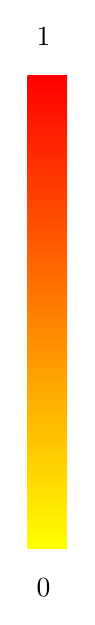
\begin{tikzpicture}[scale=1.0,auto,swap]
    \shade[top color=red,bottom color=yellow] (0,0) rectangle (0.5,6);
    \node[inner sep=0] (corr_text) at (0.2,6.5) {1};
    \node[inner sep=0] (corr_text) at (0.2,-0.5) {0};
  \end{tikzpicture}
  \caption{cluster1}
\end{figure}


\begin{figure}[H]
  \centering
  %\begin{subfigure}[b]{0.15\textwidth}
    \begin{tikzpicture}[scale=1.0,auto,swap]

    % the two brain figures on top
    \node (upper_brain) at (0,1.5) { \includegraphics*[scale=\scaleBrainImg,trim=0 0 240 0]{images/cluster2_2/stage_6.eps}};
    \node (lower_brain) at (0,-1.5) { \includegraphics*[scale=\scaleBrainImg,trim=240 0 0 0]{images/cluster2_2/stage_6.eps}};

    % the 6 circles
    \draw[fill=col200_2] (-1.6,-3.4) circle [radius=0.33cm] node {\scriptsize A};
    \draw[fill=col201_2] (-0.7,-3.4) circle [radius=0.33cm] node {\scriptsize P};
    \draw[fill=col202_2] (0.2,-3.4) circle [radius=0.33cm] node {\scriptsize T};
    \draw[fill=col203_2] (-1.6,-4.2) circle [radius=0.33cm] node {\scriptsize C1};
    \draw[fill=col204_2] (-0.7,-4.2) circle [radius=0.33cm] node {\scriptsize C2};
    \draw[fill=col205_2] (0.2,-4.2) circle [radius=0.33cm] node {\scriptsize C3};

    % the big circle on the right
    \draw[fill=col206_2] (1.3,-3.8) circle [radius=0.6cm] node {\scriptsize FDG};

    \end{tikzpicture}
  %\end{subfigure}
  % next subfigure
  \hspace{-1.5em}
  ~
  %\begin{subfigure}[b]{0.15\textwidth}
    \begin{tikzpicture}[scale=1.0,auto,swap]

    % the two brain figures on top
    \node (upper_brain) at (0,1.5) { \includegraphics*[scale=\scaleBrainImg,trim=0 0 240 0]{images/cluster2_2/stage_12.eps}};
    \node (lower_brain) at (0,-1.5) { \includegraphics*[scale=\scaleBrainImg,trim=240 0 0 0]{images/cluster2_2/stage_12.eps}};

    % the 6 circles
    \draw[fill=col210_2] (-1.6,-3.4) circle [radius=0.33cm] node {\scriptsize A};
    \draw[fill=col211_2] (-0.7,-3.4) circle [radius=0.33cm] node {\scriptsize P};
    \draw[fill=col212_2] (0.2,-3.4) circle [radius=0.33cm] node {\scriptsize T};
    \draw[fill=col213_2] (-1.6,-4.2) circle [radius=0.33cm] node {\scriptsize C1};
    \draw[fill=col214_2] (-0.7,-4.2) circle [radius=0.33cm] node {\scriptsize C2};
    \draw[fill=col215_2] (0.2,-4.2) circle [radius=0.33cm] node {\scriptsize C3};

    % the big circle on the right
    \draw[fill=col216_2] (1.3,-3.8) circle [radius=0.6cm] node {\scriptsize FDG};

    \end{tikzpicture}
  %\end{subfigure}
  % next subfigure
  \hspace{-1.5em}
  ~
  %\begin{subfigure}[b]{0.15\textwidth}
    \begin{tikzpicture}[scale=1.0,auto,swap]

    % the two brain figures on top
    \node (upper_brain) at (0,1.5) { \includegraphics*[scale=\scaleBrainImg,trim=0 0 240 0]{images/cluster2_2/stage_18.eps}};
    \node (lower_brain) at (0,-1.5) { \includegraphics*[scale=\scaleBrainImg,trim=240 0 0 0]{images/cluster2_2/stage_18.eps}};

    % the 6 circles
    \draw[fill=col220_2] (-1.6,-3.4) circle [radius=0.33cm] node {\scriptsize A};
    \draw[fill=col221_2] (-0.7,-3.4) circle [radius=0.33cm] node {\scriptsize P};
    \draw[fill=col222_2] (0.2,-3.4) circle [radius=0.33cm] node {\scriptsize T};
    \draw[fill=col223_2] (-1.6,-4.2) circle [radius=0.33cm] node {\scriptsize C1};
    \draw[fill=col224_2] (-0.7,-4.2) circle [radius=0.33cm] node {\scriptsize C2};
    \draw[fill=col225_2] (0.2,-4.2) circle [radius=0.33cm] node {\scriptsize C3};

    % the big circle on the right
    \draw[fill=col226_2] (1.3,-3.8) circle [radius=0.6cm] node {\scriptsize FDG};

    \end{tikzpicture}
  %\end{subfigure}
  % next subfigure
  \hspace{-1.5em}
  ~
  %\begin{subfigure}[b]{0.15\textwidth}
    \begin{tikzpicture}[scale=1.0,auto,swap]

    % the two brain figures on top
    \node (upper_brain) at (0,1.5) { \includegraphics*[scale=\scaleBrainImg,trim=0 0 240 0]{images/cluster2_2/stage_24.eps}};
    \node (lower_brain) at (0,-1.5) { \includegraphics*[scale=\scaleBrainImg,trim=240 0 0 0]{images/cluster2_2/stage_24.eps}};

    % the 6 circles
    \draw[fill=col230_2] (-1.6,-3.4) circle [radius=0.33cm] node {\scriptsize A};
    \draw[fill=col231_2] (-0.7,-3.4) circle [radius=0.33cm] node {\scriptsize P};
    \draw[fill=col232_2] (0.2,-3.4) circle [radius=0.33cm] node {\scriptsize T};
    \draw[fill=col233_2] (-1.6,-4.2) circle [radius=0.33cm] node {\scriptsize C1};
    \draw[fill=col234_2] (-0.7,-4.2) circle [radius=0.33cm] node {\scriptsize C2};
    \draw[fill=col235_2] (0.2,-4.2) circle [radius=0.33cm] node {\scriptsize C3};

    % the big circle on the right
    \draw[fill=col236_2] (1.3,-3.8) circle [radius=0.6cm] node {\scriptsize FDG};

    \end{tikzpicture}
  %\end{subfigure}
  % next subfigure
  \hspace{-1.5em}
  ~
  %\begin{subfigure}[b]{0.15\textwidth}
    \begin{tikzpicture}[scale=1.0,auto,swap]

    % the two brain figures on top
    \node (upper_brain) at (0,1.5) { \includegraphics*[scale=\scaleBrainImg,trim=0 0 240 0]{images/cluster2_2/stage_36.eps}};
    \node (lower_brain) at (0,-1.5) { \includegraphics*[scale=\scaleBrainImg,trim=240 0 0 0]{images/cluster2_2/stage_36.eps}};

    % the 6 circles
    \draw[fill=col240_2] (-1.6,-3.4) circle [radius=0.33cm] node {\scriptsize A};
    \draw[fill=col241_2] (-0.7,-3.4) circle [radius=0.33cm] node {\scriptsize P};
    \draw[fill=col242_2] (0.2,-3.4) circle [radius=0.33cm] node {\scriptsize T};
    \draw[fill=col243_2] (-1.6,-4.2) circle [radius=0.33cm] node {\scriptsize C1};
    \draw[fill=col244_2] (-0.7,-4.2) circle [radius=0.33cm] node {\scriptsize C2};
    \draw[fill=col245_2] (0.2,-4.2) circle [radius=0.33cm] node {\scriptsize C3};

    % the big circle on the right
    \draw[fill=col246_2] (1.3,-3.8) circle [radius=0.6cm] node {\scriptsize FDG};

    \end{tikzpicture}
  %\end{subfigure}
  % next subfigure
  \hspace{-1.5em}
  ~
  \hspace{1em}
  % the red-to-yellow gradient on the right
  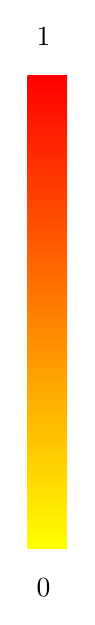
\begin{tikzpicture}[scale=1.0,auto,swap]
    \shade[top color=red,bottom color=yellow] (0,0) rectangle (0.5,6);
    \node[inner sep=0] (corr_text) at (0.2,6.5) {1};
    \node[inner sep=0] (corr_text) at (0.2,-0.5) {0};
  \end{tikzpicture}
  \caption{cluster2}
\end{figure}


\begin{figure}[H]
  \centering
  %\begin{subfigure}[b]{0.15\textwidth}
    \begin{tikzpicture}[scale=1.0,auto,swap]

    % the two brain figures on top
    \node (upper_brain) at (0,1.5) { \includegraphics*[scale=\scaleBrainImg,trim=0 0 240 0]{images/cluster3_2/stage_6.eps}};
    \node (lower_brain) at (0,-1.5) { \includegraphics*[scale=\scaleBrainImg,trim=240 0 0 0]{images/cluster3_2/stage_6.eps}};

    % the 6 circles
    \draw[fill=col300_2] (-1.6,-3.4) circle [radius=0.33cm] node {\scriptsize A};
    \draw[fill=col301_2] (-0.7,-3.4) circle [radius=0.33cm] node {\scriptsize P};
    \draw[fill=col302_2] (0.2,-3.4) circle [radius=0.33cm] node {\scriptsize T};
    \draw[fill=col303_2] (-1.6,-4.2) circle [radius=0.33cm] node {\scriptsize C1};
    \draw[fill=col304_2] (-0.7,-4.2) circle [radius=0.33cm] node {\scriptsize C2};
    \draw[fill=col305_2] (0.2,-4.2) circle [radius=0.33cm] node {\scriptsize C3};

    % the big circle on the right
    \draw[fill=col306_2] (1.3,-3.8) circle [radius=0.6cm] node {\scriptsize FDG};

    \end{tikzpicture}
  %\end{subfigure}
  % next subfigure
  \hspace{-1.5em}
  ~
  %\begin{subfigure}[b]{0.15\textwidth}
    \begin{tikzpicture}[scale=1.0,auto,swap]

    % the two brain figures on top
    \node (upper_brain) at (0,1.5) { \includegraphics*[scale=\scaleBrainImg,trim=0 0 240 0]{images/cluster3_2/stage_12.eps}};
    \node (lower_brain) at (0,-1.5) { \includegraphics*[scale=\scaleBrainImg,trim=240 0 0 0]{images/cluster3_2/stage_12.eps}};

    % the 6 circles
    \draw[fill=col310_2] (-1.6,-3.4) circle [radius=0.33cm] node {\scriptsize A};
    \draw[fill=col311_2] (-0.7,-3.4) circle [radius=0.33cm] node {\scriptsize P};
    \draw[fill=col312_2] (0.2,-3.4) circle [radius=0.33cm] node {\scriptsize T};
    \draw[fill=col313_2] (-1.6,-4.2) circle [radius=0.33cm] node {\scriptsize C1};
    \draw[fill=col314_2] (-0.7,-4.2) circle [radius=0.33cm] node {\scriptsize C2};
    \draw[fill=col315_2] (0.2,-4.2) circle [radius=0.33cm] node {\scriptsize C3};

    % the big circle on the right
    \draw[fill=col316_2] (1.3,-3.8) circle [radius=0.6cm] node {\scriptsize FDG};

    \end{tikzpicture}
  %\end{subfigure}
  % next subfigure
  \hspace{-1.5em}
  ~
  %\begin{subfigure}[b]{0.15\textwidth}
    \begin{tikzpicture}[scale=1.0,auto,swap]

    % the two brain figures on top
    \node (upper_brain) at (0,1.5) { \includegraphics*[scale=\scaleBrainImg,trim=0 0 240 0]{images/cluster3_2/stage_18.eps}};
    \node (lower_brain) at (0,-1.5) { \includegraphics*[scale=\scaleBrainImg,trim=240 0 0 0]{images/cluster3_2/stage_18.eps}};

    % the 6 circles
    \draw[fill=col320_2] (-1.6,-3.4) circle [radius=0.33cm] node {\scriptsize A};
    \draw[fill=col321_2] (-0.7,-3.4) circle [radius=0.33cm] node {\scriptsize P};
    \draw[fill=col322_2] (0.2,-3.4) circle [radius=0.33cm] node {\scriptsize T};
    \draw[fill=col323_2] (-1.6,-4.2) circle [radius=0.33cm] node {\scriptsize C1};
    \draw[fill=col324_2] (-0.7,-4.2) circle [radius=0.33cm] node {\scriptsize C2};
    \draw[fill=col325_2] (0.2,-4.2) circle [radius=0.33cm] node {\scriptsize C3};

    % the big circle on the right
    \draw[fill=col326_2] (1.3,-3.8) circle [radius=0.6cm] node {\scriptsize FDG};

    \end{tikzpicture}
  %\end{subfigure}
  % next subfigure
  \hspace{-1.5em}
  ~
  %\begin{subfigure}[b]{0.15\textwidth}
    \begin{tikzpicture}[scale=1.0,auto,swap]

    % the two brain figures on top
    \node (upper_brain) at (0,1.5) { \includegraphics*[scale=\scaleBrainImg,trim=0 0 240 0]{images/cluster3_2/stage_24.eps}};
    \node (lower_brain) at (0,-1.5) { \includegraphics*[scale=\scaleBrainImg,trim=240 0 0 0]{images/cluster3_2/stage_24.eps}};

    % the 6 circles
    \draw[fill=col330_2] (-1.6,-3.4) circle [radius=0.33cm] node {\scriptsize A};
    \draw[fill=col331_2] (-0.7,-3.4) circle [radius=0.33cm] node {\scriptsize P};
    \draw[fill=col332_2] (0.2,-3.4) circle [radius=0.33cm] node {\scriptsize T};
    \draw[fill=col333_2] (-1.6,-4.2) circle [radius=0.33cm] node {\scriptsize C1};
    \draw[fill=col334_2] (-0.7,-4.2) circle [radius=0.33cm] node {\scriptsize C2};
    \draw[fill=col335_2] (0.2,-4.2) circle [radius=0.33cm] node {\scriptsize C3};

    % the big circle on the right
    \draw[fill=col336_2] (1.3,-3.8) circle [radius=0.6cm] node {\scriptsize FDG};

    \end{tikzpicture}
  %\end{subfigure}
  % next subfigure
  \hspace{-1.5em}
  ~
  %\begin{subfigure}[b]{0.15\textwidth}
    \begin{tikzpicture}[scale=1.0,auto,swap]

    % the two brain figures on top
    \node (upper_brain) at (0,1.5) { \includegraphics*[scale=\scaleBrainImg,trim=0 0 240 0]{images/cluster3_2/stage_36.eps}};
    \node (lower_brain) at (0,-1.5) { \includegraphics*[scale=\scaleBrainImg,trim=240 0 0 0]{images/cluster3_2/stage_36.eps}};

    % the 6 circles
    \draw[fill=col340_2] (-1.6,-3.4) circle [radius=0.33cm] node {\scriptsize A};
    \draw[fill=col341_2] (-0.7,-3.4) circle [radius=0.33cm] node {\scriptsize P};
    \draw[fill=col342_2] (0.2,-3.4) circle [radius=0.33cm] node {\scriptsize T};
    \draw[fill=col343_2] (-1.6,-4.2) circle [radius=0.33cm] node {\scriptsize C1};
    \draw[fill=col344_2] (-0.7,-4.2) circle [radius=0.33cm] node {\scriptsize C2};
    \draw[fill=col345_2] (0.2,-4.2) circle [radius=0.33cm] node {\scriptsize C3};

    % the big circle on the right
    \draw[fill=col346_2] (1.3,-3.8) circle [radius=0.6cm] node {\scriptsize FDG};

    \end{tikzpicture}
  %\end{subfigure}
  % next subfigure
  \hspace{-1.5em}
  ~
  \hspace{1em}
  % the red-to-yellow gradient on the right
  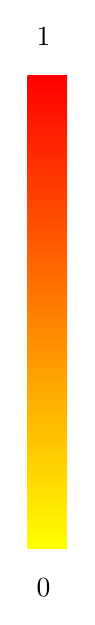
\begin{tikzpicture}[scale=1.0,auto,swap]
    \shade[top color=red,bottom color=yellow] (0,0) rectangle (0.5,6);
    \node[inner sep=0] (corr_text) at (0.2,6.5) {1};
    \node[inner sep=0] (corr_text) at (0.2,-0.5) {0};
  \end{tikzpicture}
  \caption{cluster3}
\end{figure}



% scale parameter for the font size in the circles
\newcommand*{\scaleLabelImg}{0.7}
\begin{figure}[H]
  \centering
  {\scalefont{\scaleLabelImg}
  \begin{tikzpicture}[scale=1.0,auto,swap]

  % the two brain figures on top
  \node (brain) at (0,1.5) { \includegraphics*[scale=\scaleLabelImg]{images/Mid-Lateral_surface3.eps}};

  % the 6 circles
  \draw[scale=\scaleLabelImg] (-9,-6) circle [radius=2cm] node {ABETA142};
  \draw[scale=\scaleLabelImg] (-4,-6) circle [radius=2cm] node {PTAU181P};
  \draw[scale=\scaleLabelImg] (1,-6) circle [radius=2cm] node {TAU};
  \draw[scale=\scaleLabelImg] (-9,-10.5) circle [radius=2cm] node {RAVLT};
  \draw[scale=\scaleLabelImg] (-4,-10.5) circle [radius=2cm] node {MMSE};
  \draw[scale=\scaleLabelImg] (1,-10.5) circle [radius=2cm] node {ADAS13};

  % the big circle on the right
  \draw[scale=\scaleLabelImg] (8,-8.25) circle [radius=4cm] node {FDG-PET};

  \end{tikzpicture}
  }

  \caption{Labels of the different areas analysed}
\end{figure}

\end{document}

